\chapter{StochasticNet: Forming Deep Neural Networks via Stochastic Connectivity}

{\small \textbf{Authors}\\
MOHAMMAD JAVAD SHAFIEE, (Student Member, IEEE), PARTHIPAN SIV, AND ALEXANDER WONG, (Senior Member, IEEE)\\ \\
IEEE ACCESS\\VOLUME 4, 2016}

\section{Proposed Method}

This is going to be the last paper we will be discussing in this report and what we want to do is to make a comparison between the following proposed method and some regularization tecniques. So far we have mentioned many times Dropout and Batch Normalization as well as DisturbLabel and most likely something else. The important thing to point out is that with StochasticNet (which is the name of the proposed network) we are not talking about a specific regularization tecnique but as there are a few things in common it is actually possible to make a comparison. Before of going any further it would make sense to introduce the topic from which the StochasticNet comes from and it is the theory by which a neural network can be represented as a random graph. Obviously in this graph there are many constraints as it is not possible to have that neurons in a layer are connected with neurons of non-adjacent layers, and moreover, as we are presenting a stochastic network, it must be clear that when we create a connection between two nodes (or neurons) there is a constraint that shall be such that the weight is between 0 and 1. So we look at weights as if they were probabilities. What we can do in StochasticNets is to set a value that represents the sparsity (the probability by which is possible to create a connection) we are looking for and then we can understand how different performance is when testing the network on some datasets. But we will compare these things in the following section. The important thing is to understand that while with a regularization tecnique such as Dropout we temporarily ``freeze'' the values of the weights (by setting them to zero) during the training step, here with StochasticNet we start with a sparse network and finish with a sparse network. In fact, after a regularization tecnique is employed, it is applied only in the training step. When the training is done, we resume the frozen weights and use the full network with the test set. That does not happen with StochasticNet. In order to get a better idea, we show in Figure \ref{fig:10_2} the several phases of a model through different regularization tecniques and of course StochasticNet.\\

\begin{figure}[h!]
    \centering
    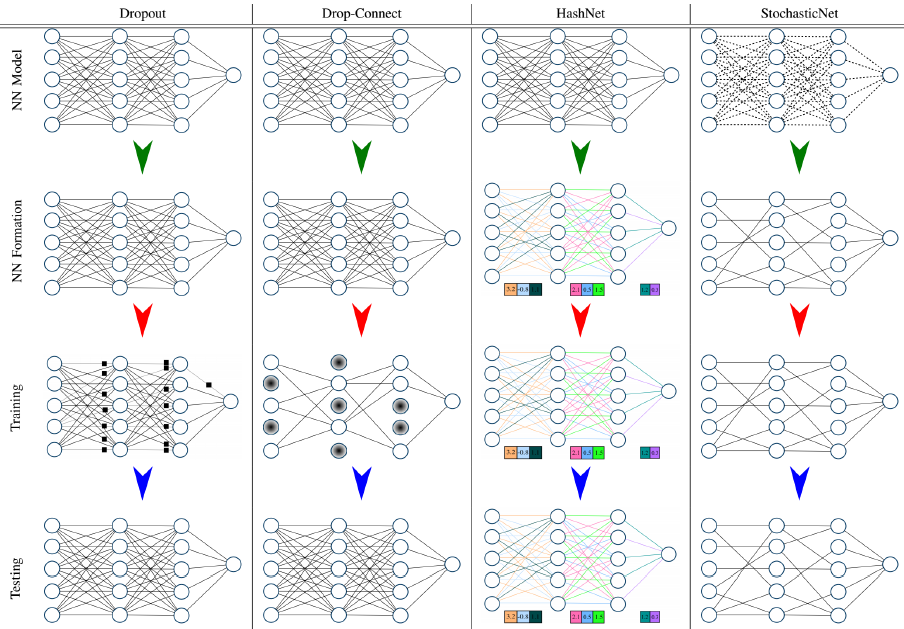
\includegraphics[scale=0.60]{images/10_2.png}
    \caption{Comparison among several stochastic regularization methods and StochasticNet.}
    \label{fig:10_2}
\end{figure}

\FloatBarrier

\section{Experimental Results}

Experimental results have been evaluated on the following datasets: CIFAR-10 \citep{CIFAR10and100}, MNIST \citep{MNIST}, SVHN \citep{SVHN} and STL-10 \citep{STL10}. After having performed a few tests it turns out that StochasticNet achieves the same test error of a conventional CNN but with far fewer connections. In fact, it is estimated that we have around half of the connections. Moreover, we can justify the following results as in the convolution, we perform the dot product between the filter and the matrix with a sparsified matrix. On the other hand in an ordinary CNN we have a non-sparse matrix. That is why it can be translated into a very good improvement, even though a degradation of our performance is obtained once we go below the 39\% of connectivity. But it seems to be quite reasonable and it still confirms the effectiveness of this network.